%%%%%%%%%%%%%%%%%%%%%%%%%%%%%%%%%%%%%%%%%%%%%%%%%%%%%%%%%%%%%%%%%%%%
% Diskussion und Ausblick
%%%%%%%%%%%%%%%%%%%%%%%%%%%%%%%%%%%%%%%%%%%%%%%%%%%%%%%%%%%%%%%%%%%%
\onehalfspacing
\chapter{Outlook}
  \label{Outlook}

\section{Trello Alfred Extension}\index{Trello}\index{Alfred!Extension}

Alfred \cite{alfred}\index{Alfred} is a small Mac\index{Mac} application which simplifies the way one can search the web or access all sorts of applications. It constist just of a input field which one cann access with a keystroke combination. It's like an extended Spotlight (on Mac\index{Mac}) or Windows Search\index{Windows!Search} (on Windows). Developers can write extensions to access other webservices and applications with Alfred\index{Alfred}. It's even possible to run scripts with Alfred\index{Alfred}. With that possibility given it's perfect for acessing Trello while working in a fast and easy way. 



There are three commands to add or read cards with this extension:

\begin{enumerate}
	\item \texttt{trello board-name} will return the card-names and statuses of this board.
	\item \texttt{trello board-name list-name} will return card-names and statuses of this list in this board.
	\item \texttt{trello board-name text for a new card} will add a new card with the specified text to the first list of this board.
	\item \texttt{trello board-name list-name text for a new card} will add a new card with the specified text to this list of this board.
\end{enumerate}

If you enter \texttt{trello Berlin Visit the Reichstag} in Alfred\index{Alfred} the extension looks for a board called \emph{Berlin}. If it finds nothign it looks for \emph{Berlin Visit} and so on. So your board names shouldn't end with an imperative. The thought behind this operating principle is that it's very unlikely that a board name ends with an imperative and that imperatives are often used for card titles because cards are sort of a command.

\begin{figure}[htb]
\centering
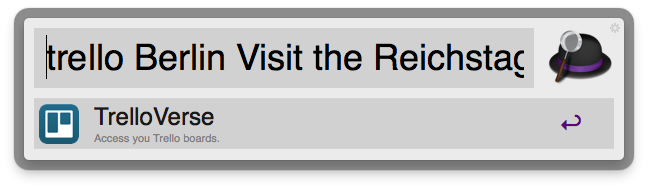
\includegraphics[width=\textwidth]{figures/trello-ext.png}
\caption{Alfred Extension\index{Alfred!Extension} for Trello\index{Trello}: This command would add a card with the name \emph{Visit the Reichstag} to the board called \emph{Berlin}.}
\label{fig:trello-ext}
\end{figure}

If you omit the text after the board name the extension will show you all card names of this board and its statuses.

Sometimes there are several boards with similar board names. In this case the extension will pick the \textquotedblleft last\textquotedblright match. So if you have two boards called \emph{Berlin} and \emph{Berlin sightseeing} the extension will would pick \emph{Berlin sightseeing}. This approach makes sense because if the extension would pick the first match, in this case \emph{Berlin}, it wouldn't be possible to access \emph{Berlin sightseeing}. In the case that one wants to access \emph{Berlin} and add a new card beginning with \emph{sightseeing} one has to put this board name betweet tick marks.

\todo{Maybe code it and verify practicability.}

\section{Native applications}
Although Trello is an extremely good web-app, I'm of the opinion that a native application is always the better solution. The first reason is because it's a dedicated app and so it's integrated with the operationg system. Especially for to-do-applications it's an advantage that they can access the systems notification system, or that they could completely vanish in the background so they don't bother the user while working. There are mobile applications for iOS\index{iOS} \cite{trello:ios} and Android\index{Android} \cite{trello:android} by Trello itself. But theres no Mac\index{Mac}, Windows\index{Windows} or Linux\index{Linux} application.

A native application would even speed up the Alfred\index{Alfred} extension because the application could cache the data. So there hasn't to be an actual HTTP request for every command by the Alfred extension. And if a HTTP request necessary the user hasn't to wait because the application will handle the command in the background.